\documentclass{article}
% translate with >> pdflatex -shell-escape <file>

% This file is used as unit test for pgfplots, copyright by Christian Feuersaenger.
% 
% See
%   http://pgfplots.sourceforge.net/pgfplots.pdf
% for pgfplots.
%
% Any required input files (for <plot table> or <plot file> or the table package) can be downloaded
% at
% http://www.ctan.org/tex-archive/graphics/pgf/contrib/pgfplots/doc/latex/
% and
% http://www.ctan.org/tex-archive/graphics/pgf/contrib/pgfplots/doc/latex/plotdata/

\usepackage{pgfplots}
\pgfplotsset{compat=newest}

\pagestyle{empty}

\begin{document}
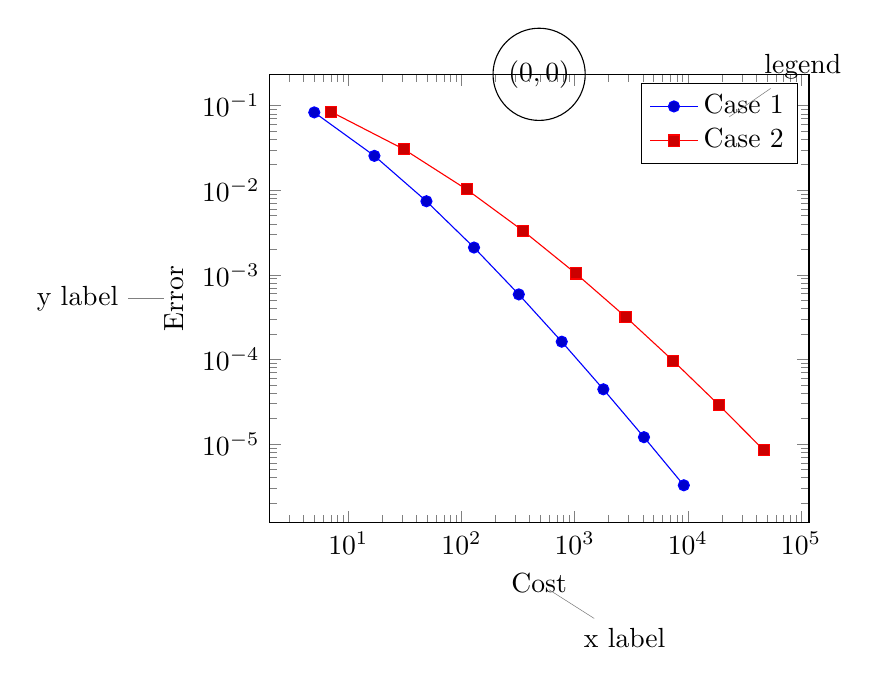
\begin{tikzpicture}[baseline]%
	\node[circle,draw=black] at (0,0) {$(0,0)$};
	\begin{loglogaxis}[
		anchor=north,
		name=firstplot,
		xlabel=Cost,
		ylabel=Error,
		y label style={name=myylabel},
		x label style={name=myxlabel},
		legend style={name=mylegend,
			row 1 column 2/.style={blue,name=firstentry}% doesn't work!
		}
	]
	\addplot plot coordinates {
		(5,     8.31160034e-02)
		(17,    2.54685628e-02)
		(49,    7.40715288e-03)
		(129,   2.10192154e-03)
		(321,   5.87352989e-04)
		(769,   1.62269942e-04)
		(1793, 4.44248889e-05)
		(4097, 1.20714122e-05)
		(9217, 3.26101452e-06)
	};
	\addplot plot coordinates {
		(7,     8.47178381e-02)
		(31,    3.04409349e-02)
		(111,   1.02214539e-02)
		(351,   3.30346265e-03)
		(1023,  1.03886535e-03)
		(2815,  3.19646457e-04)
		(7423,  9.65789766e-05)
		(18943, 2.87339125e-05)
		(47103, 8.43749881e-06)
	};
	\legend{Case 1\\Case 2\\}
	\end{loglogaxis}

	\node[pin=45:legend] at (mylegend.center) {};
	\node[pin=-45:x label] at (myxlabel.center) {};
	\node[pin=180:y label] at (myylabel.center) {};
\end{tikzpicture}
\end{document}
